\section{Headbanger System Design}\label{sec:design}

In this section, we explain how the Headbanger system authenticates smart glass users by monitoring their head movement patterns. In order to make head movement natural for users, we play (fast beat) music track and record the accelerometer readings while users move their head following the music rhythm. As such, authenticating a user involves comparing her sensor readings with the pre-recorded glass owner's sensor readings\footnote{In this section, we assume there is only one owner per glass, and we can easily extend our scheme to handle the cases with multiple owners.}. Figure~\cite{***} shows the design detail of the Headbanger system.

%Finally, we note that such a method can be easily extended to authenticating other wearable devices such as smart watches (by monitoring arm/hand movement).

***SL: need a whole picture of the algorithm**


\subsection{Collecting and Preprocessing Sensor Samples}

To facilitate natural head movement, we provide several short music tracks with easy-to-follow beats. Users may choose one of these songs and move their head along the rhythm for $T$ seconds. During the duration of $T$ seconds, we record the built-in accelerometer sensor readings (with sampling rate of $r$) into a $30r $ matrix, which we refer to as one $ACC$ sample. We hypothesize that head-movement can serve as a reliable behavioral biometric -- that is, $ACC$ samples from the same user have smaller distances than samples from different users.


We first need to preprocess the raw samples before we can accurately quantify the similarity between any two samples. Figure~\ref{fig:freq_resp} shows five users' $ACC$ samples in frequency domain. The diagrams show that most of the frequencies fall between 0 and 5 Hz. In addition, we note that most of the music tracks have *** beats per second, hence head-movement frequency lower than ***Hz. As a result, we filter raw $ACC$ samples by adopting a low pass Butterworth filter~\cite{***} with a high cutoff frequency of 10Hz. The resulting accelerometer data is thus smoother and suitable for further processing.



\begin{figure}[t]
\centering
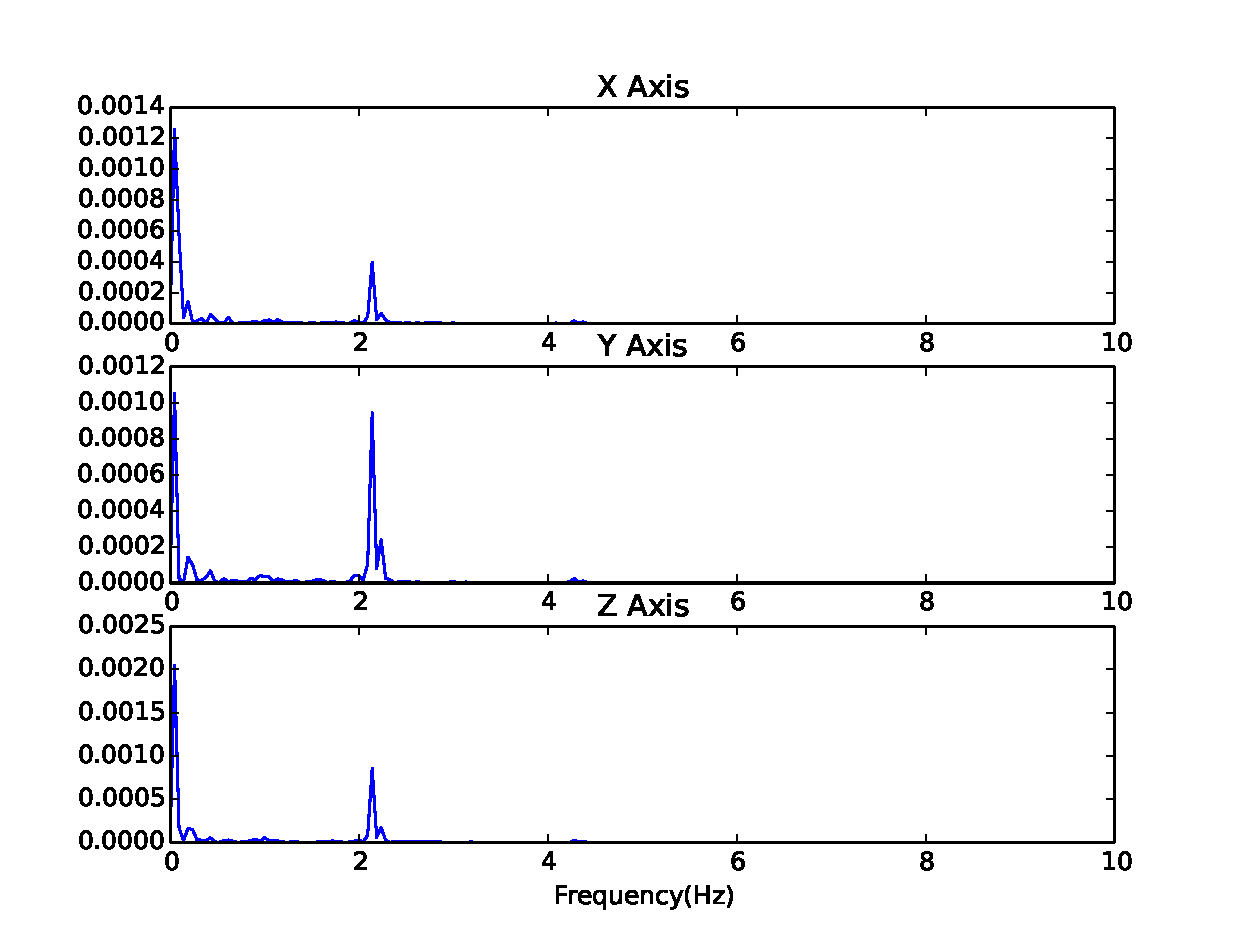
\includegraphics [width=.95\linewidth]{fig/freq_resp.eps}
\caption{\label{fig:freq_resp}Fiver users' $ACC$ samples in frequency domain.}
\end{figure}

\subsection{Quantifying Sample Similarity}

Next we investigate how we can accurately quantify the similarity level between two $ACC$ samples, whose results will be used to classify the users. After testing various methods (e.g., ***), we decide to adopt the Dynamic Time Warping (DTW) algorithm~\cite{***} that is often used to measure similarity between two waves based on temporal stimulation.  Unlike many other algorithms, DTW measures the similarity between two signals that are similar but with phase difference, which is well suited for our study. In our study, users often start head movement at a different angle, but exhibit similar, often periodic, pattern for a similar amount of time. Applying the DTW algorithm on two $ACC$ samples $S1, S2$, we get a vector $(d_x, d_y, d_z)$ denoting the distance in the $x, y, z$ axes respectively. DTW is expected to return relatively small distance values for samples from the same user, while returning large distance values for samples from different users (that have different movement patterns).

***YZ: Sugang, we need some detailed equations or algorithms here. ***





\subsection{Classifying Users}

In this study, we consider two ways of classifying smart device users, with the first one using support vector machine (SVM) while the second one using a simple thresholding scheme. Below we discuss these two methods in more detail.

\subsubsection{SVM-Based Classification}

In SVM-based classification, we construct the training set by including both ``true'' samples from the glass owner and ``false'' samples from a number of random users. We then calculate the DTW vectors between any two true samples (with the resulting DTW vectors referred to as $DTW_{T\rightarrow T}$), as well as DTW vectors between any true sample and false sample (with the resulting DTW vectors referred to as $DTW_{T\rightarrow F}$). Given a testing sample $S$, we calculate the DTW vectors between $S$ and any true sample (with the resulting vectors referred to as $DTW_{S\rightarrow T}$) as well as DTW vectors between $S$ and false samples (with the resulting vectors referred to as $DTW_{S\rightarrow F}$). Finally, we input both training DTW vectors (i.e., $DTW_{T\rightarrow T}$ and $DTW_{T\rightarrow F}$) and testing DTW vectors (i.e., $DTW_{S\rightarrow T}$ and $DTW_{S\rightarrow F}$) to the support vector machine, which will return the classification result -- $1$ means the user is accepted as the owner while $0$ means the user is rejected.

In order to minimize the computing overhead in the above process and make it suitable for running on a smart glass, we propose the following optimization: instead of looking at every single training sample from a user, we choose a few representative samples and use them for classification. Here, we define a user's representative samples as those that are the most similar to the rest of her samples. Suppose a user's entire training set has $N$ samples. For every sample, we compute its distance to each of the $N-1$ samples using DTW. Then we choose the $K$ samples that have the lowest $K$ average distance to the rest of the training set, hence the most representative samples. We refer to these $K$ samples as top $K$ samples of the user. If we choose a small $K$ value, say 3, the computing overhead will be significantly reduced.



\begin{eqnarray}
DTWave(n) = \frac{\sum_{i\neq{n}}DTW_i(n)}{N} \\
DTWave_e = min\{DTWave_1,...,DTWave_N\}
\label{eq:top1}
\end{eqnarray}


%In the testing phase, given a testing sample, we calculate its distance to each training set's top $K$ samples. Suppose we have $K$ true training samples, and $fK$ false training sets ($f$ is the number of false training sets), then we will have $(f+1)K$ distance values for the testing sample. We then input these distance values to the SVM classifier which will return the classification result -- $1$ means the user is classified as the owner while $o$ means the user is not classified as the owner.


\subsubsection{Thresholding-Based Classification}

One potential problem with SVM is that it is not robust against false training samples that happen to be close to true training samples. Alternatively, we consider a thresholding-based classification scheme, in which we only focus on true training samples. Given $N$ true training samples, we first identify the top $K$ samples, and calculate their DTW vectors to the rest of the samples. As a result, we have $(N-1)K$ distance vectors in total. We then calculate the mean $\mu$ and standard deviation $\sigma$ of these values, and define the ``true'' range as $[\mu-m\sigma, \mu+m\sigma]$.

In the testing phase, given a testing sample, we calculate the DTW distance between the testing sample and the top $K$ training samples. If the resulting distance mean falls into the true range, then the user is accepted as the owner; otherwise, the user is rejected.

